\appendix
\section{Artifact Appendix}

\textbf{All commands are relative to the repository root.}

\begin{enumerate}
\item \textbf{Regression suite (software sanity).}
\begin{verbatim}
python -m pytest -q
\end{verbatim}
Expected: exit code 0. (Preflight logs are recorded under \texttt{build/paperA\_preflight\_out\_v4/}.)

\item \textbf{Independent consistency check (anti-circularity support).}
\begin{verbatim}
python tools/independent_check.py --paperA
\end{verbatim}
Expected: exit code 0 (no independent consistency errors). Logs under \texttt{build/paperA\_preflight\_out\_v4/}.

\item \textbf{Software gate (audit).}
\begin{verbatim}
python tools/audit_min.py --mode software
\end{verbatim}
Expected: exit code 0 and JSON \texttt{decision=="GO"}.

\item \textbf{Bit-exactness verifier on core benchmarks (golden \texorpdfstring{$\leftrightarrow$}{<->} C++ reference).}
\begin{verbatim}
python -m nema bench verify benches/B1_small/manifest.json \
--outdir build/paper_verify/b1

python -m nema bench verify benches/B3_kernel_302_7500/manifest.json \
--outdir build/paper_verify/b3
\end{verbatim}
Expected (PASS) for each run: verifier JSON reports \texttt{ok==true} and \texttt{mismatches==[]} (i.e., mismatch=0).

\item \textbf{External bundle workflow (B4).}
\begin{verbatim}
python -m nema bench verify benches/B4_real_connectome/manifest.json \
--outdir build/paper_verify/b4
\end{verbatim}
Expected (PASS): verifier completes with \texttt{ok==true}. Contract expectation: referenced external files exist; if sha256 is not a placeholder token, it must match the file digest.

\item \textbf{Hardware pipeline generation (HLS + Vivado evidence capture).}
\begin{verbatim}
bash tools/run_hw_gates.sh
\end{verbatim}
Expected (PASS by artifact contract): \texttt{build\_hw/} contains at least one \texttt{**/bench\_report.json} and report files under \texttt{**/hw\_reports/**/*.(rpt|xml|log)} (or the equivalent set consumed by the report parser).

\item \textbf{Hardware gate (audit).}
\begin{verbatim}
python tools/audit_min.py --mode hardware
\end{verbatim}
Expected (PASS): exit code 0 and JSON contains \texttt{decision=="GO"}; criteria include \texttt{hardwareToolchainAvailable=True}, \texttt{hardwareEvidenceG0b=True}, \texttt{hardwareEvidenceG2=True}, \texttt{hardwareEvidenceG3=True}, and \texttt{digestMatchAll=True}.

\item \textbf{Regenerate paper-facing tables/figures/evidence (refresh the pack).}
\begin{verbatim}
python tools/paperA/build_review_pack_v3.py
\end{verbatim}
Expected: updates the paper tables (\texttt{results\_bitexact.csv}, \texttt{results\_qor.csv}, \texttt{results\_throughput.csv}) and the coverage report (\texttt{vivado\_coverage\_report.md}) under \texttt{papers/paperA/artifacts/}, and refreshes the preflight outputs directory.

\item \textbf{Build the PDF.}
\begin{verbatim}
make -C papers/paperA clean paper
\end{verbatim}
Expected: exit code 0; paper PDF produced at \texttt{papers/paperA/text/paper.pdf}.

\item \textbf{Sanity-check the pre-generated gate snapshot.}
\begin{verbatim}
cat papers/paperA/artifacts/tables/gates_summary.md
cat papers/paperA/artifacts/figures/gates_status.txt
\end{verbatim}
Expected: \texttt{gates\_summary.md} shows both software and hardware with \texttt{decision=GO}; \texttt{gates\_status.txt} exists.

\item \textbf{Optional (ergonomics; not a scientific claim): checkpoint/bundle regeneration.}
\begin{verbatim}
bash tools/checkpoint_full.sh
\end{verbatim}
Expected: produces an evidence bundle and/or updated evidence directory consistent with the repository's checkpoint conventions.
\end{enumerate}

\subsection{Artifact Snapshot (pre-generated assets)}

The appendix directly references the current artifact files in \texttt{papers/paperA/artifacts/}.

\begin{figure}[h]
\centering
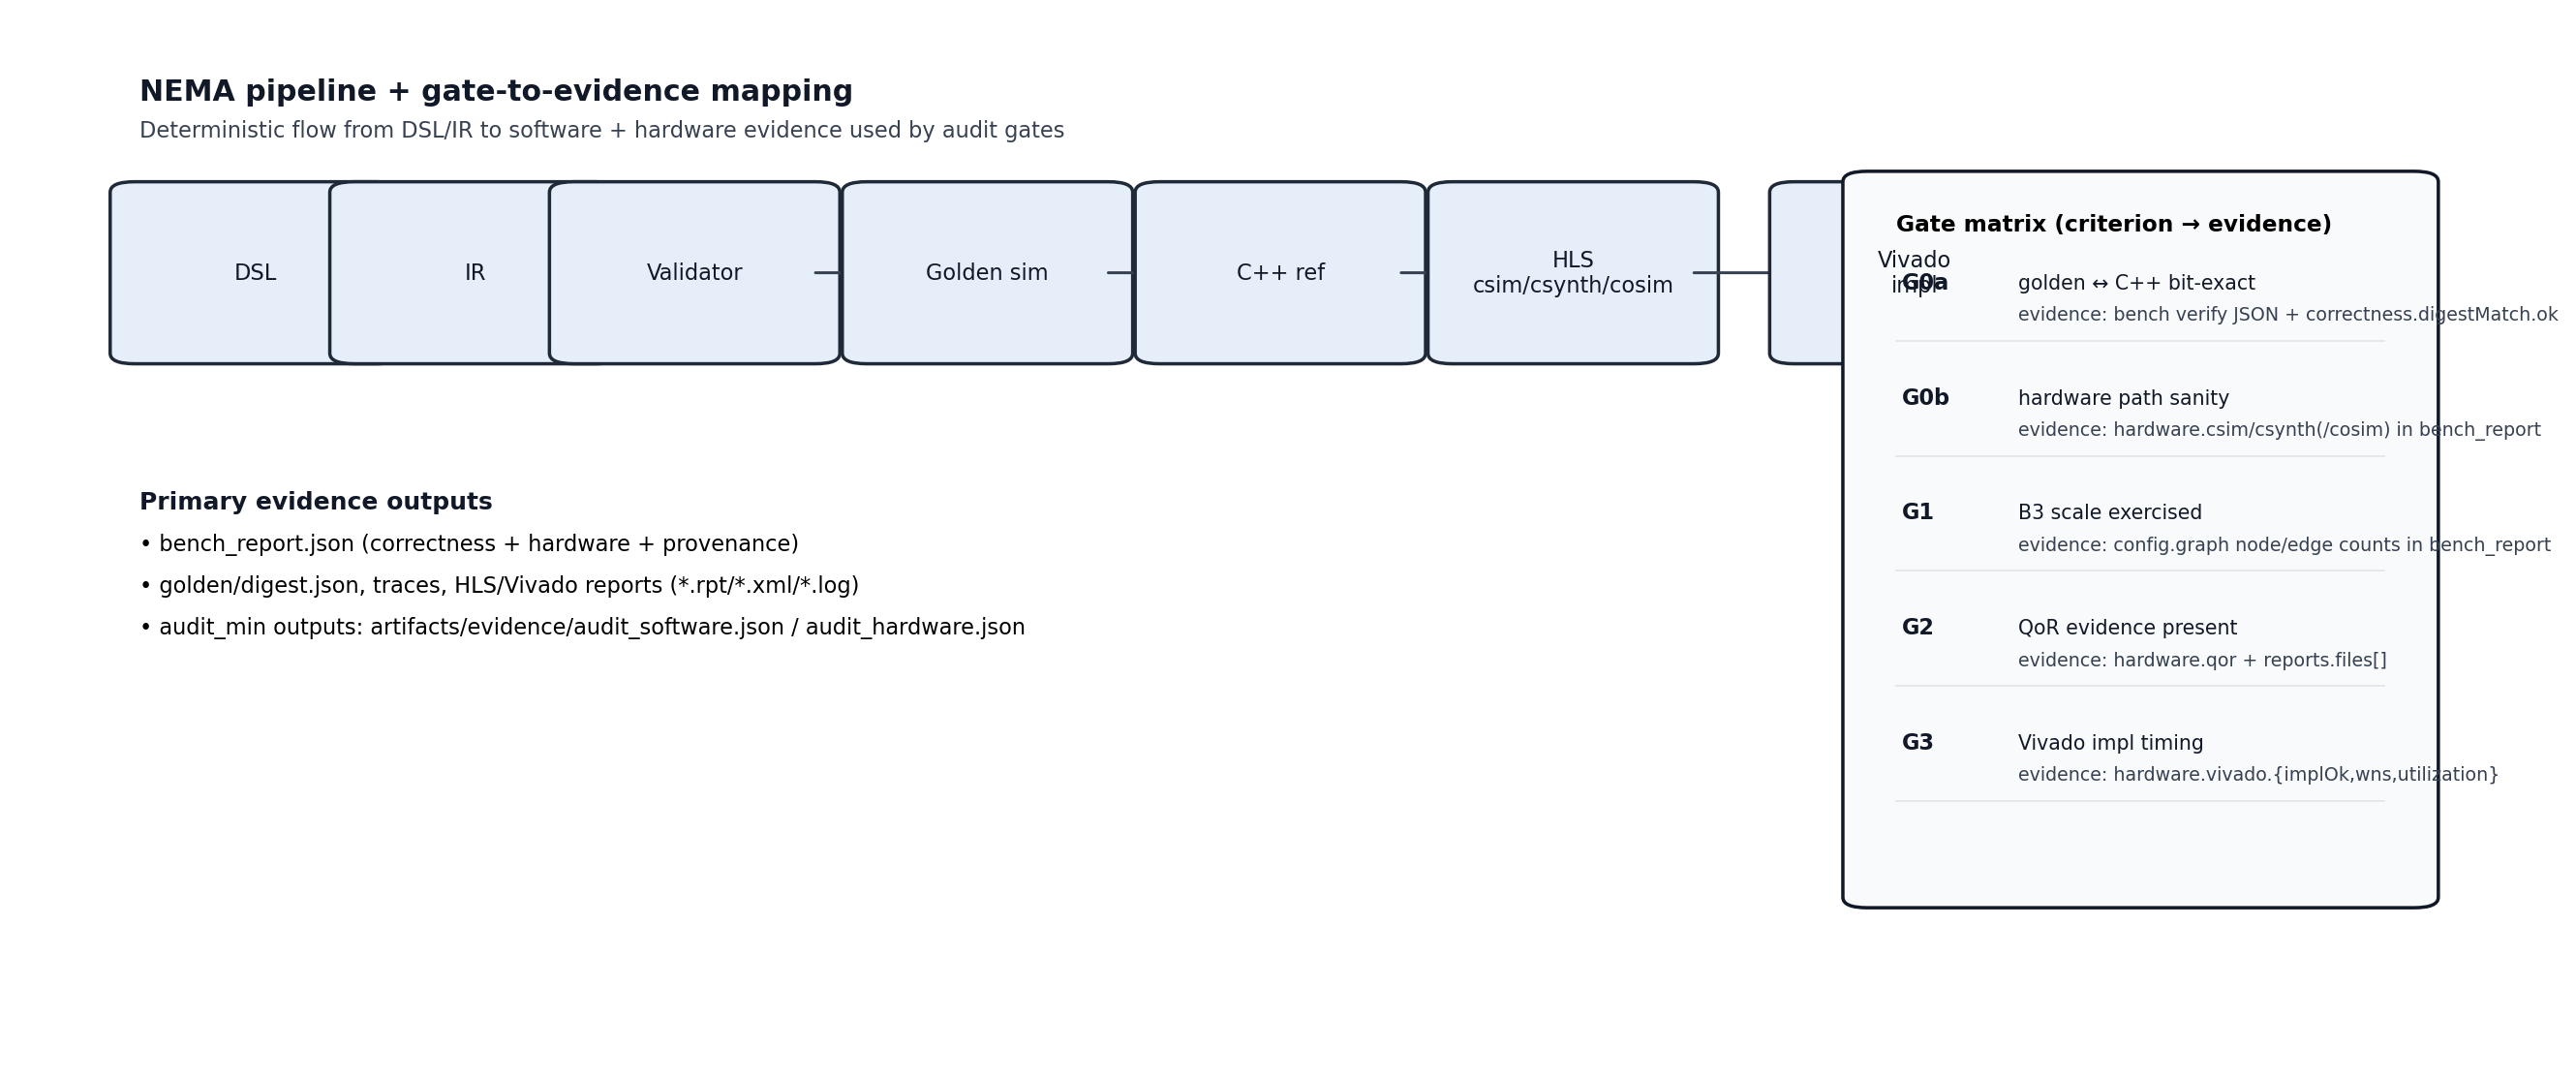
\includegraphics[width=0.98\linewidth]{../artifacts/figures/fig_pipeline_gates.png}
\caption{NEMA pipeline and gate-to-evidence mapping. G0a validates bit-exactness between golden and C++ reference (\texttt{bench verify} / \texttt{correctness.digestMatch.ok}); G0b validates hardware-path execution evidence (\texttt{csim/csynth/cosim} fields in \texttt{bench\_report.json}); G1 validates that the 302/7500 benchmark evidence is present; G2 validates QoR/report evidence (\texttt{hardware.qor} and report files); G3 validates Vivado implementation timing/utilization evidence (\texttt{hardware.vivado.*}). Gate outputs and decisions are recorded in \texttt{papers/paperA/artifacts/evidence/audit\_software.json} and \texttt{papers/paperA/artifacts/evidence/audit\_hardware.json}.}
\label{fig:pipeline-gates}
\end{figure}

\paragraph{Legacy status snapshot.}
\texttt{papers/paperA/artifacts/figures/gates\_status.txt} is retained as a lightweight artifact snapshot, but Figure~\ref{fig:pipeline-gates} is the primary evidence-facing figure used by the paper.
